
\فصل{روش پیشنهادی}

فصل حاضر به شرح مراحل عملیاتی پروژه اختصاص دارد.
در این بخش ابتدا نحوه‌ی آماده‌سازی مجموعه‌داده شرح داده می‌شود.
سپس بررسی می‌شود که این تصاویر دستخوش چه تغییراتی شده و چگونه به مدل ورودی داده می‌شوند.
در ادامه، طراحی انجام‌شده برای مدل یادگیری ماشین توصیف می‌شود.
بخش انتهایی این بخش نیز به ذکر 
جزئیات فرایند آموزش مدل و مقدمه‌ای بر فرایند آزمایش مدل خواهد گذشت.

\قسمت{آماده‌سازی مجموعه‌داده}

داده‌هایی که از مراکز پزشکی دریافت می‌شوند، مسیر طولانی‌ای را طی می‌کنند تا برای آموزش مدل قابل استفاده باشند.
اولین مرحله‌ی این آماده‌سازی شامل نگاشت اطلاعات بیماران به تصاویر می‌باشد.
این نگاشت از طریق شماره‌ی شناسه‌ی بیمار صورت می‌گیرد 
و در نتیجه‌ی آن، اطلاعات پزشکی در دسترس از بیماران به همراه مسیر ذخیره‌سازی تصاویر وی به صورت ساخت‌یافته‌ای جمع‌آوری می‌شوند.\

مرحله‌ی بعد، جداسازی تصاویر مورد توجه پژوهش است.
تصویربرداری‌های انجام‌شده از بیماران، معمولا تنها شامل مغز نمی‌شوند و تصاویری از ریه و \dots را نیز در بر دارند.
به علاوه در هر مجموعه، تعداد تصاویر مغزی نیز با مجموعه‌های دیگر می‌تواند تفاوت داشته باشد.
به گونه‌ای که یک بیمار ۱۵ و بیمار دیگر، ۵۰ برش از مغز را در مجموعه‌ی خود داشته باشد.
این در حالی است که در امتیازدهی ASPECT تنها چند برش خاص از مغز مورد استفاده قرار می‌گیرد.
به این ترتیب، یکی از گام‌های ضروری برای آماده‌سازی داده‌ها، جداسازی این برش‌ها از میان تمام 
تصاویر دریافت‌شده از بیماران و تهیه‌ی یک نگاشت مدون از هر بیمار به برش‌های استخراج‌شده از تصاویر وی می‌باشد.\\

با انجام دو اقدام فوق که بیشتر مربوط به مرتب‌سازی و خالص‌سازی اطلاعات بودند، نوبت به مرحله‌ی پیش‌پردازش
\footnote{Preprocessing}
تصاویر می‌رسد.
پیش‌پردازش یکی از مهم‌ترین و موثرترین گام‌های یادگیری ماشین محسوب می‌شود که ارتباط مستقیمی با عملکرد و توانایی یادگیری مدل دارد. 
درواقع پیش‌پردازش شامل تغییراتی در داده‌های ورودی است که باعث می‌شود تا جای ممکن، اطلاعات نامفید از داد‌ه‌ها حذف شوند و اطلاعات کلیدی نیز در قالب مناسبی به مدل عرضه شوند.
به این ترتیب فرایند یادگیری برای مدل ساده‌تر خواهد بود.
نکته‌ی دیگری که باعث اهمیت بیش‌تر پیش‌پردازش می‌شود، قابلیت استفاده‌ی مجدد آن در پژوهش‌های دیگر است.
درواقع گام پیش‌پردازش تصاویر پزشکی در بسیاری از پژوهش با هم اشتراکات زیادی دارد.
روش‌های ارائه شده در این پروژه نیز می‌توانند در پیش‌پردازش تصاویر CT در سایر تحقیقات راهگشا باشند.
در ادامه، فرایند پیش‌پردازش مورد استفاده در این پژوهش، به صورت گام به گام بر روی یک تصویر مغزی انتخابی شرح داده می‌شوند.

\subsection{افزایش وضوح}
همانطور که در بخش مفاهیم اولیه ذکر شد، مقدار عددی هر پیکسل در تصاویر پزشکی، بازه‌ی بزرگی را شامل می‌شود.
این در حالی است که چشم انسان تنها تعداد محدودی رنگ خاکستری را می‌تواند از هم تمیز دهد.
به همین دلیل، در صورت مشاهده‌ی یک تصویر CT خام، جزئیات بافت مغز و حتی ناحیه‌ی آسیب‌دیده، قابل مشاهده نخواهد بود. 
با این توضیح، تصویر انتخابی برای شرح مراحل پیش‌پردازش، در ابتدا مانند 
شکل \ref{fig:raw-ct} است.
\footnote{ناحیه‌ی مغز برای مقاصد نمایشی، کمی جا‌به‌جا شده‌است.}
بنابراین، در اولین گام، لازم است وضوح تصاویر افزایش داده‌شود.\\

\begin{figure}[ht]
\centering
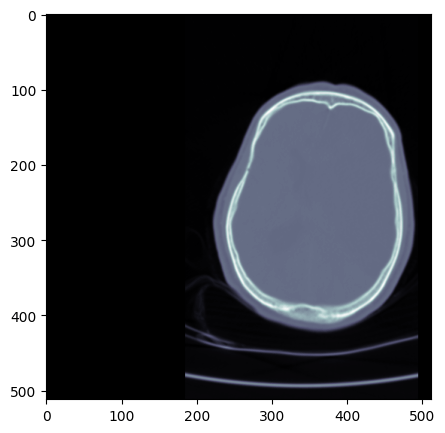
\includegraphics[width=\textwidth, keepaspectratio]{raw-ct.png}
\caption[]{تصویر انتخابی برای نمایش مراحل پیش‌پردازش، در حالت اولیه.}
\label{fig:raw-ct}
\end{figure}

 میان مقدار هر پیکسل با بافت یا شیئی که نمایش می‌دهد ارتباط وجود دارد.
به نحوی که آب، مقدار $0 HU$، هوا مقدار $-1000 HU$، بافت استخوانی مقدار $1000 HU$ و بافت مغزی در حدود $20-50 HU$ می‌باشد.
% Chapter 1 - Computed tomography imaging and angiography – principles
% Author links open overlay panelShervin Kamalian 1, Michael H. Lev 2, Rajiv Gupta 1
به این ترتیب، با محدود کردن مقدار پیکسل‌ها به بازه‌ای مثل $0-100 HU$، اطلاعات مربوط به بافت مغز از بین نمی‌رود.
اما این بار به علت کاهش بازه‌ی رنگ خاکستری، اجزای تصویر از هم بهتر تمایز می‌یابند.
در اصطلاح تصاویر پزشکی، به بازه‌ای که مقادیر به آن محدود می‌شوند پهنای پنجره 
\footnote{Window Width}
و به مرکز این بازه سطح پنجره 
\footnote{Window Level} گفته می‌شود.
با اعمال پهنای پنجره‌ی 100 و سطح پنجره‌ی ۵۰، تصویر اولیه مانند شکل 
\ref{fig:windowed-image}
می‌شود.\\

\begin{figure}[ht]
\centering
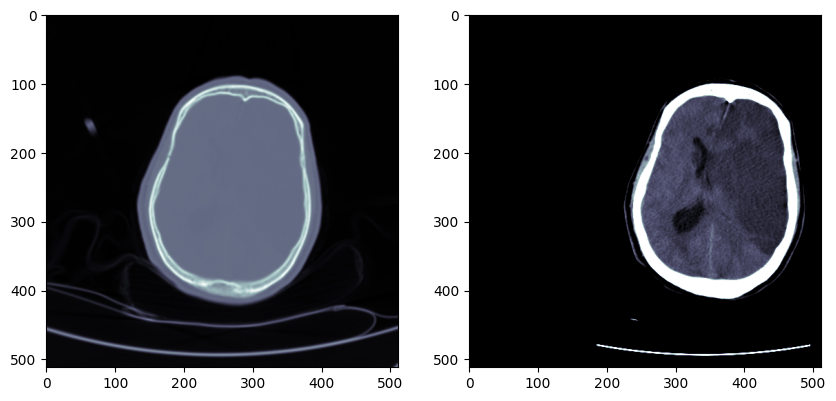
\includegraphics[width=\textwidth, keepaspectratio]{windowed-ct.png}
\caption[]{تصویر انتخابی برای نمایش مراحل پیش‌پردازش، پس از تنظیم پهنای پنجره به 100 و سطح پنجره به ۵۰.}
\label{fig:windowed-ct}
\end{figure}

روش معمول برای افزایش وضوح تصاویر، به همین صورت با تنظیم پهنا و سطح پنجره می‌باشد.
اما باید توجه داشت که میان تصاویر بیماران مختلف، تفاوت‌های جزئی وجود دارد.
برخی تصاویر ممکن است به طور کلی قدری تیره‌تر و یا روشن‌تر باشند.
در نتیجه اعمال یک سیاست واحد برای پهنا و سطح پنجره ممکن است برای تمام تصاویر، بهینه نباشد و وضوح لازم را برای تصویر فراهم نکند.
در این پژوهش، از یک روش پویا برای تنظیم وضوح تصاویر استفاده شده‌است که شرح آن در ادامه می‌آید.\\

در این روش، ابتدا مقدار پیکسل‌های مربوط به بافت مغزی هر بیمار به صورت یک مجموعه، استخراج می‌شوند.
سپس چند درصد پایین و چند درصد بالای این مقادیر محاسبه می‌شوند.
در نتیجه، یک چندک
\footnote{quantile} 
پایین و یک چندک بالا به‌دست می‌آید.
در نهایت، مقادیر پیکسل‌های کل تصویر، محدود به بازه‌ی میان این دو چندک می‌شوند.
به این ترتیب، در هر تصویری، با توجه به اطلاعات آماری همان تصویر، 
مقدار پیکسل‌ها محدود به بازه‌ای از رنگ خاکستری می‌شود که اطلاعات بیش‌تری در خود دارد.
اعمال این روش پویا، نیازمند استخراج بافت مغزی است که در مراحل انتهایی پیش‌پردازش به‌دست می‌آید.
به همین جهت، از آوردن تصویر آن در این بخش صرف نظر می‌شود
اما تصویر نهایی فرایند پیش‌پردازش، نمایانگر افزایش بیشتر وضوح 
تصاویر نسبت به روش‌های ایستا (مانند تصویر \ref{fig:windowed-ct}) می‌باشد.\\
